\section{Access Control Design Model}
\begin{figure}[H]
  \centering
  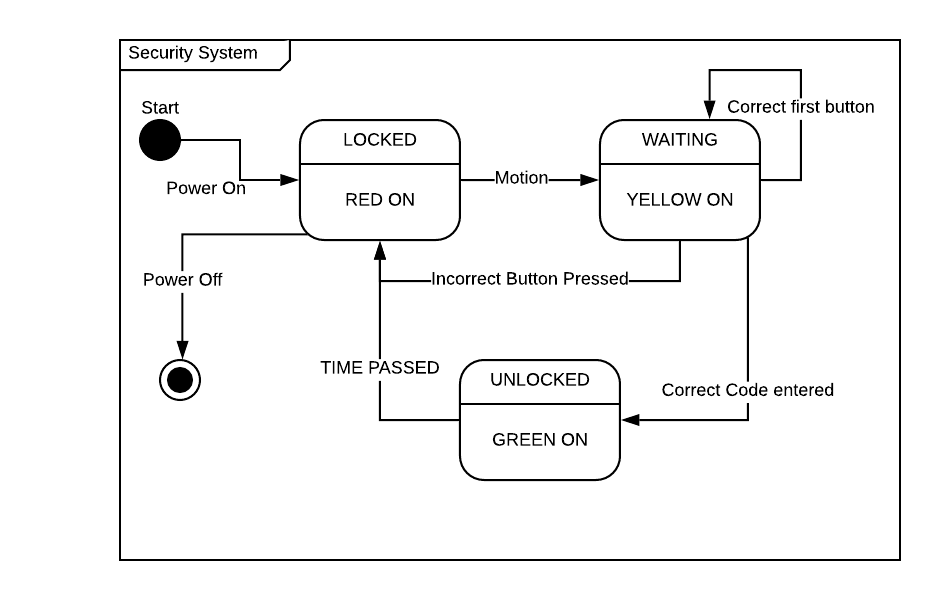
\includegraphics[scale=0.75]{figs/StateMachine.png}
  \caption{Access Control State Machine}
  \label{fig:StateMachine}
\end{figure}
The state machine models the functionality the final system has available. It does not actually have any locking or protection in place. Extending the system to accept longer and safer codes should not be hard, and connecting a solenoid or actuator to physically lock something would probably be easy. 

The machine has 3 discrete states: 
\begin{itemize}
  \item \textbf{Locked} \\
The system starts in this state, it also enters it 10 seconds after entering the unlocked state.
In this state the Red LED light is on. And whatever the system is protecting should be unavailable.
  \item \textbf{Waiting}\\
The system enters this state from the Locked state when the PIR detector senses movement. 
The Yellow LED will be lit while waiting. 
The system will wait in this state until a code sequence is entered. It will move the system to the Unlocked state when the two correct buttons are pressed in sequence. The yellow LED will blink whenever a button is pressed. It will move to the Locked state whenever a wrong key is pressed compared to what was required.
  \item \textbf{Unlocked}\\
The system enters this state from the Waiting state after a correct code has been entered. In this state the Green LED will stay lit. 
The system will exit this state after 10 seconds and then enter the Locked state again. 
\end{itemize}

As the state machine is a model to help with writing the code we didn't model the blinking of the Yellow LED light whenever buttons are pressed. 
\pagebreak